
\documentclass[a4paper]{article}
\usepackage{pdflscape}
%Tutti gli usepackage vanno qui

\usepackage{geometry}
\usepackage[italian]{babel}
\usepackage[utf8]{inputenc}
\usepackage[T1]{fontenc}
\usepackage{tabularx}
\usepackage{longtable}
\usepackage{hyperref}
\usepackage{enumitem}
\hypersetup{
	colorlinks=true,
	linkcolor=black,
	filecolor=magenta,      
	urlcolor=blue,
}
% Numerazione figure 
\let\counterwithout\relax
\let\counterwithin\relax
\usepackage{chngcntr}

\counterwithin{table}{subsection}
\counterwithin{figure}{subsection}

\usepackage[bottom]{footmisc}
\usepackage{fancyhdr}
\usepackage{titlesec}
\setcounter{secnumdepth}{4}
\usepackage{amsmath, amssymb}
\usepackage{array}
\usepackage{graphicx}

%\usepackage{float}
\usepackage{layouts}
\usepackage{float}
\usepackage{eurosym}


\usepackage{layouts}
\usepackage{float}
\usepackage{eurosym}

%Comandi di impaginazione uguale per tutti i documenti
\pagestyle{fancy}
\lhead{
\includegraphics[scale=0.07]{res/images/logo8_crop.png}}
%Titolo del documento
\rhead{\doctitle{}}
\rfoot{\thepage}
\cfoot{}
\setlength{\headheight}{35pt}
\setcounter{tocdepth}{4}
\setcounter{secnumdepth}{4}
\renewcommand{\footrulewidth}{0.4pt}

% multirow per tabelle
\usepackage{multirow}

% Permette tabelle su più pagine

%\usepackage{longtable}


% colore di sfondo per le celle
\usepackage[table]{xcolor}

%COMANDI TABELLE
\newcommand{\rowcolorhead}{\rowcolor[HTML]{56A5EC}} %intestazione 
\newcommand{\rowcolorlight}{\rowcolor[HTML]{fafafa}} %righe chiare/dispari
\newcommand{\rowcolordark}{\rowcolor[HTML]{e1f5fe}} %righe scure/pari
\newcommand{\colorhead}{\color[HTML]{FFFFFF}} %testo intestazione
\newcommand{\colorbody}{\color[HTML]{000000}} %testo righe
\newcommand{\tabitem}{~~\rlap{\textbullet}~~}

\newcommand{\glo}{$_{G}$}
\newcommand{\glosp}{$_{G}$ }

\definecolor{pari}{HTML}{E1F5
\definecolor{dispari}{HTML}{FAFAFA}


%Lista dei comandi personalizzati
\newcommand{\doctitle}{Verbale interno 2019-02-20}
\newcommand{\rev}{1.0.0}
\newcommand{\approv}{}
\newcommand{\ver}{}
\newcommand{\red}{Matteo Santinon}
\newcommand{\stato}{Approvato}
\newcommand{\uso}{Interno}
\newcommand{\describedoc}{Riassunto dell'incontro del gruppo \textit{8Lab 
Solutions} tenutosi il 2019-02-20.}
\newcommand{\destinatari}{8Lab Solutions\\& Prof. Tullio Vardanega\\& Prof. Riccardo Cardin}



\usepackage{listings}
\usepackage{color}

\definecolor{dkgreen}{rgb}{0,0.6,0}
\definecolor{gray}{rgb}{0.5,0.5,0.5}
\definecolor{mauve}{rgb}{0.58,0,0.82}
%define Javascript language
\lstdefinelanguage{JavaScript}{
	keywords={typeof, new, true, false, catch, function, return, null, catch, switch, var, if, in, while, do, else, case, break, then, deployer, deploy, artifacts, require},
	keywordstyle=\color{blue}\bfseries,
	ndkeywords={class, export, boolean, throw, implements, import, this},
	ndkeywordstyle=\color{darkgray}\bfseries,
	identifierstyle=\color{black},
	sensitive=false,
	comment=[l]{//},
	morecomment=[s]{/*}{*/},
	commentstyle=\color{purple}\ttfamily,
	stringstyle=\color{red}\ttfamily,
	morestring=[b]',
	morestring=[b]"
}
\lstset{
	language=JavaScript,
	extendedchars=true,
	basicstyle=\footnotesize\ttfamily,
	showstringspaces=false,
	showspaces=false,
	numbers=left,
	numberstyle=\footnotesize,
	numbersep=9pt,
	tabsize=2,
	breaklines=true,
	showtabs=false,
	captionpos=b
}



\makeindex
\begin{document}
\thispagestyle{empty}
\begin{titlepage}
	\begin{center}
		
\includegraphics[scale = 0.3]{res/images/logo8_crop.png}\\
		\large \textbf{8Lab Solutions - Progetto "Soldino"} \\
		\vfill
		\Huge \textbf{\doctitle}
		\vspace*{\fill}
        
        \vfill
        \large
        \begin{tabular}{r|l}
                        \textbf{Versione} & \rev{} \\
                        \textbf{Approvazione} & \approv{} \\
                        \textbf{Redazione} & \red{} \\
                        \textbf{Verifica} & \ver{} \\
                        \textbf{Stato} & \stato{} \\
                        \textbf{Uso} & \uso{} \\
                        \textbf{Destinato a} & \parbox[t]{5cm}{8Lab Solutions
                        \\Prof. Tullio Vardanega\\Prof. Riccardo Cardin}
                \end{tabular}
                \vfill
                \normalsize
                \textbf{Descrizione}\\
                \describedoc
                \vfill
                \small
                \texttt{8labsolutions@gmail.com}
	\end{center}
\end{titlepage}


\pagebreak
\section*{Changelog}
\renewcommand{\arraystretch}{1.5}
\rowcolors{2}{pari}{dispari}
	\begin{longtable}{ 
			>{\centering}p{0.09\textwidth} 
			>{\centering}p{0.13\textwidth}
			>{\centering}p{0.2\textwidth} 
			>{\centering}p{0.16\textwidth} 
			>{}p{0.2775\textwidth} }
		
		\rowcolorhead
		\textbf{\color{white}Version} & 
		\textbf{\color{white}Date} & 
		\textbf{\color{white}Name} & 
		\textbf{\color{white}Role} &
		\centering \textbf{\color{white}Description} 
		\tabularnewline  
		\endfirsthead
		\rowcolorhead
		\textbf{\color{white}Version} & 
		\textbf{\color{white}Date} & 
		\textbf{\color{white}Name} & 
		\textbf{\color{white}Role} &
		\centering \textbf{\color{white}Description} 
		\tabularnewline  
		\endhead
		
		1.0.0 & 2019-03-30 & PLACEHOLDER & \textbf{Project Manager} &
		Approval
		\tabularnewline
		
		0.2.0 & 2019-03-27 & PLACEHOLDER & \textbf{Verifier} &
		Verification
		\tabularnewline
		
		0.1.2 & 2019-03-25 & PLACEHOLDER & \textbf{RUOLO} &
		Written §5.3, §5.4 and §6
		\tabularnewline
		
		0.1.2 & 2019-03-25 & PLACEHOLDER & \textbf{RUOLO} &
		Written §4.4 and §4.5
		\tabularnewline
		
		0.1.1 & 2019-03-24 & PLACEHOLDER & \textbf{RUOLO} &
		Written §3.3 and §4.3
		\tabularnewline
		
		0.1.0 & 2019-03-22 & PLACEHOLDER & \textbf{Verifier} &
		Verification
		\tabularnewline
		
		0.0.4 & 2019-03-21 & PLACEHOLDER & \textbf{RUOLO} &
		Written §3.2, §4.2 and §5.2
		\tabularnewline
		
		0.0.3 & 2019-03-21 & PLACEHOLDER & \textbf{RUOLO} &
		Written §3.1, §4.1 and §5.1
		\tabularnewline
		
		0.0.2 & 2019-03-20 & PLACEHOLDER & \textbf{RUOLO} &
		Written §1 and §2
		\tabularnewline
		
		0.0.1 & 2019-03-20 & Federico Bicciato & 
		\textbf{RUOLO} & Created document's structure.
		\tabularnewline
		
	
	\end{longtable}
\renewcommand{\arraystretch}{1} 


\pagebreak
\tableofcontents

\pagebreak
\listoffigures

\pagebreak
\listoftables

\pagebreak
\section{Introduction} 
\subsection{Manual contents}
This document is the developer manual of he project \textit{Soldino}, developed by the team \textit{8Lab Solutions} for the proponent \textit{Red Babel}.\newline
Within the manual you can find:
\begin{itemize}
	\item the technologies used for the development;
	\item the software tools used and suggested;
	\item the software architecture;
	\item the architectural and design pattern used;
	\item the functionalities provided by \textit{Soldino}.
\end{itemize}

\subsection{Purpose of the manual}
The contents of the manual are intended to help the developers who decide to 
maintain or further develop \textit{Soldino}. Everything described here can 
help the developer to fully and deeply understand the design, use and features 
of the application, so that it can be modified and improved with ease.\newline
Many technologies, tools and languages are used to build the app: these are 
only briefly explained in their parts that cover the application domain. 
Additional references can be found in the "Reference" section.

\subsection{Purpose of the product}
The platform \textit{Soldino} is a DApp accessible on a web browser as a 
client interface and the plug-in Metamask as a virtual wallet.\newline
The main functionality of \textit{Soldino} is trading goods and services 
online. Since the platform's backend is coded on the Ethereum blockchain, it 
provides more security and transparency than the traditional e-commerce 
websites.\newline
The platform is built to be managed by the government. The currency used is 
called Cubit, and it's a ERC20 compliant fork of Ether, minted and managed by 
the government itself.

\subsection{References}
	\begin{itemize}
		\item \textbf{Ganache} \url{https://truffleframework.com/ganache}
		\item \textbf{Git} \url{https://it.atlassian.com/git}
		\item \textbf{Node.js} \url{https://nodejs.org/it/}
		\item \textbf{Node Package Manager} \url{https://www.npmjs.com/get-npm}
		\item \textbf{Surge.sh} \url{https://surge.sh/help/getting-started-with-surge}
		\item \textbf{Truffle} \url{https://truffleframework.com/truffle}
		\item \textbf{Solidity} \url{https://solidity.readthedocs.io/en/v0.5.0/}
	\end{itemize}

\pagebreak
\section{Setup} 
\subsection{Requirements}
In this section we describe all the requirements needed.
\subsubsection{Browser}
Soldino is accessible through a web interface. The currently most recent versions of the following broswers are supported:
\begin{itemize}
	\item \textbf{Mozilla Firefox}: version 66.0.1;
	\item \textbf{Google Chrome} version 73.0.3683.86.
\end{itemize}

\subsubsection{Tools}
The following tools are needed:
\begin{itemize}
	\item \textbf{Node.js}: you need it to run commands and as a Truffle requirement;
	\item \textbf{Truffle}: you need it to write and deploy contracts with ease;
	\item \textbf{Ganache}: you need it to put up a local Ethereum network and check transactions on it;
	\item \textbf{Metamask}: a browser plugin used as a virtual wallet.
	\item \textbf{Surge.sh}: the web platform chosen to host the website interface of Soldino.
\end{itemize}

\subsubsection{Dependencies}
Soldino depends on many different packages, some for use and others for development.\\
All these packages are located in the file \texttt{package.json} which is in the root folder of the project.\\
The packages required to execute the software \textit{Soldino} are listed below.\\

\renewcommand{\arraystretch}{1.5}
\rowcolors{2}{pari}{dispari}
\begin{longtable}{ 
		>{\centering}p{0.4\textwidth} 
		>{\centering}p{0.4\textwidth}
	}
	\caption{Packages required for software usage}\\
	\rowcolorhead
	\textbf{\color{white}Software} & 
	\textbf{\color{white}Version}
	\tabularnewline  
	\endhead	
	
	% voci prese da package.json, repo "Soldino-PoC, ramo "develop"


	react-text-mask & $\geq$5.4.4
	\tabularnewline
	commondir &$\geq$1.0.1
	\tabularnewline
	history &$\geq$4.7.2
	\tabularnewline
	prop-types &$\geq$15.7.2\tabularnewline
	react &$\geq$16.8.3\tabularnewline
	react-dom &$\geq$16.8.3\tabularnewline
	react-number-format &$\geq$4.0.6\tabularnewline
	react-redux &$\geq$6.0.1\tabularnewline
	react-router &$\geq$4.3.1\tabularnewline
	react-router-dom &$\geq$4.3.1\tabularnewline
	react-router-redux &$\geq$4.0.8\tabularnewline
	react-scripts &$\geq$2.1.8\tabularnewline
	redux &$\geq$4.0.1\tabularnewline
	redux-thunk &$\geq$2.3.0\tabularnewline
	web3 & 1.0.0-beta.37\tabularnewline
	
\end{longtable}

Other packages, listed below, are required for the development.
\renewcommand{\arraystretch}{1.5}
\rowcolors{2}{pari}{dispari}
\begin{longtable}{ 
		>{\centering}p{0.4\textwidth} 
		>{\centering}p{0.4\textwidth}
	}
	\caption{Packages required for development}\\
	\rowcolorhead
	\textbf{\color{white}Software} & 
	\textbf{\color{white}Version}
	\tabularnewline  
	\endhead	
	
	% voci prese da package.json, repo "Soldino-PoC, ramo "develop"
	eslint & 5.12.0\tabularnewline
	eslint-config-airbnb &$\geq$17.1.0\tabularnewline
	eslint-loader & $\geq$2.1.2\tabularnewline
	eslint-plugin-import & $\geq$2.16.0\tabularnewline
	eslint-plugin-jsx-a11y & $\geq$6.2.1\tabularnewline
	pre-commit & $\geq$1.2.2\tabularnewline
	truffle-contract & $\geq$4.0.6
	
\end{longtable}

\subsection{Installing}
\subsubsection{Browser}
The first thing is to have your browser installed. You can get the latest chrome version  \href{https://www.google.com/chrome/}{here}.\\

\subsubsection{Node}
Install Node.js. Digit on the shell the following commands:
\begin{enumerate}
	\item \texttt{curl -sL https://deb.nodesource.com/setup\_11.x | sudo -E bash -}
	\item \texttt{sudo apt-get install -y nodejs}
	\item check that \texttt{node} have been installed correctly with \texttt{node -v}.
\end{enumerate}
There is no need to install npm separately, since it is automatically installed with Node.

\subsubsection{Truffle}
Third thing: install Truffle.\\
Truffle requirements are:
\begin{itemize}
	\item an OS among Linux, Windows and MacOS (prefer Linux);
	\item NodeJS v8.9.4 or later (we picked version 11);
	\item Node Package Manager (npm).
\end{itemize}
You can then install Truffle with the command:
\begin{itemize}
	\item[] \texttt{npm install -g truffle}
\end{itemize}

\subsubsection{Ganache}
Fourth step: installing Ganache. There are three step to install Ganache:
\begin{enumerate}
	\item you can download the Ganache executable at this \href{https://truffleframework.com/ganache}{link}, clicking on the download button.;
	\item give the permissions to make the Ganache file executable. This can be done on Linux with the command \texttt{chmod +x path-of-the-appimage/ganache-1.3.0-x86\_64.AppImage};
	\item eventually, run it double clicking on the icon.
\end{enumerate}

\subsection{MetaMask}
MetaMask comes in the form of browser extension. You can add it to your browser this way:
\begin{itemize}
	\item Chrome:  \href{https://chrome.google.com/webstore/search/metamask?hl=it}{https://chrome.google.com/webstore/search/metamask?hl=it};
	\item Firefox: \href{https://addons.mozilla.org/it/firefox/addon/ether-metamask/?src=search}{https://addons.mozilla.org/it/firefox/addon/ether-metamask/?src=search}.
\end{itemize}

\subsection{Surge}
Install Surge.sh with the shell command
\begin{itemize}
	\item[]\texttt{npm install -g surge}.
\end{itemize}


\subsection{Configuration}
This section shows how to properly configure your work environment, so that it's the same as the one we worked on. 
This way you will hopefully encounter as little troubles as possible.\\


\subsection{Running}
Now that you have all the required software installed, it's time to get it up running.\\


\subsection{Deploying}
%not sure about this
This part shows how to deploy you contracts with Truffle and have them up running on Soldino.


\pagebreak
\section{Set up the work environment}
This chapter has the purpose to configure the work environment like our development environment, of every members of 8Lab Solutions. \\
\textbf{Note}: if you are not contributing to this project but you are only using it, it
is not necessary to follow this section of the document.
\subsection{VS Code}
We use Microsoft VS Code for writing smart contracts, for react, redux and for testing our DApp. You can download Microsoft VS Code at the following link: \url{https://code.visualstudio.com/}. We use this environment because it offers useful plugins for Solidity and linting.
\subsection{ESLint plugin}
Useful plugin for VS Code that provides linting during code typing. The extension uses the ESLint library installed in the open workspace folder.
It can be installed from the internal plug-in store (accessible with Ctrl+Shift+X),
searching ”EsLint”.
\subsection{Solidity plugin}
VS Code has a useful plugin to check Solidity syntax and lint, called ”Solidity”.
It can be installed from the internal store of the program (accessible with Ctrl+Shift+X),
searching ”JuanBlanco Solidity”.
For further info about the installation and the configuration please visit the official guide on GitHub, accessible from the following link:
https://github.com/
juanfranblanco/vscode-solidity
\subsection{React browser plugin}
To better debug React components it is recommended to use the following plugins: \\ \\
For Mozilla Firefox:
\url{https://addons.mozilla.org/it/firefox/addon/react-devtools} \\ \\
For Google Chrome:
\url{https://chrome.google.com/webstore/detail/react-developer-tools/fmkadmapgofadopljbjfkapdkoienihi}
\subsection{Redux browser plugin}
For checking Redux store and other Redux features it is recommended to use the following plugins: \\ \\
For Mozilla Firefox:
\url{https://addons.mozilla.org/it/firefox/addon/reduxdevtools/} \\ \\
For Google Chrome: \\
\url{https://chrome.google.com/webstore/detail/redux-devtools/lmhkpmbekcpmknklioeibfkpmmfibljd?hl=it}


\pagebreak
\section{Testing}
% questo cap effettivamente ha questo scopo nei 353 (2 pagine). In sostanza parla piu` di metriche che di test
This chapter shows how to
\begin{itemize}
	\item test the javascript and solidity code automatically;
	\item check if the code syntax is complied to the rules given.
\end{itemize}
\subsection{Test in Javascript Code}
%PLACEHOLDER
\subsection{Test Solidity Code}
\subsection{Code Coverage}
\textbf{Note}: Not available for Windows. \\
To run test coverage open new shell into the \textit{Soldino} project directory and run: \\ \\ \texttt{npm run coverage}. \\ \\ After a while it will show you every successfully tests and costs of transactions. The port that is used for test newtork is 8545.
% La struttura interna delle sezioni di React, Redux, Web3 e Solidity e` indicativa, non tassativa. Specie per Web3, che e` quello meno strutturato, e che i 353 non hanno descritto in questo documento

\pagebreak
\section{React} 

\subsection{Overview}
React\glosp is a JavaScript library, based on \texttt{npm} and made by Facebook, for building user interfaces by assembling user-defined components.
\subsection{Components}
Components are the core of this \texttt{npm} module. \textit{Soldino} is made of two types of component:
\begin{itemize}
	\item Presentational components;
	\item Container components.
\end{itemize}
\subsubsection{Presentational}
Each presentational component implements \texttt{Component} interface provided by the library. According to this interface, some methods are inherited from the presentational components: in particular our components uses \texttt{Render()} method to render themselves.
Most components can be customized with different parameters when they are created. These creation parameters are called \texttt{props}. Each presentational component returns a single HTML tag, here we can customize the returned tag with some Bootstrap classes. The props are accessible by the components that own them, referencing them with \texttt{this.props.propsName}.

\subsubsection{Containers} 
This type of component is like a wrapper of presentational components. A function called \texttt{Connect(arg1, arg2)} is needed for connecting a container component to a presentational component: in this way we can map some actions and some application state variables inside the presentational component, passing them through props. The \texttt{arg1} is a function called \texttt{mapStateToProps()} and the \texttt{arg2} is another function called \texttt{mapDispatchToProps()}.
\subsection{React-Router} 
React-router-dom is a \texttt{npm} module used for rendering different pages without reloading the entire website, this module works with \texttt{Render()} method provided by each presentational component. \textit{Soldino} is a single page application, so the router, implemented into a JavaScript file called \texttt{App.js}, is responsible to manage which components should be rendered.

\subsection{UML} 
\begin{figure}[H]
	\centering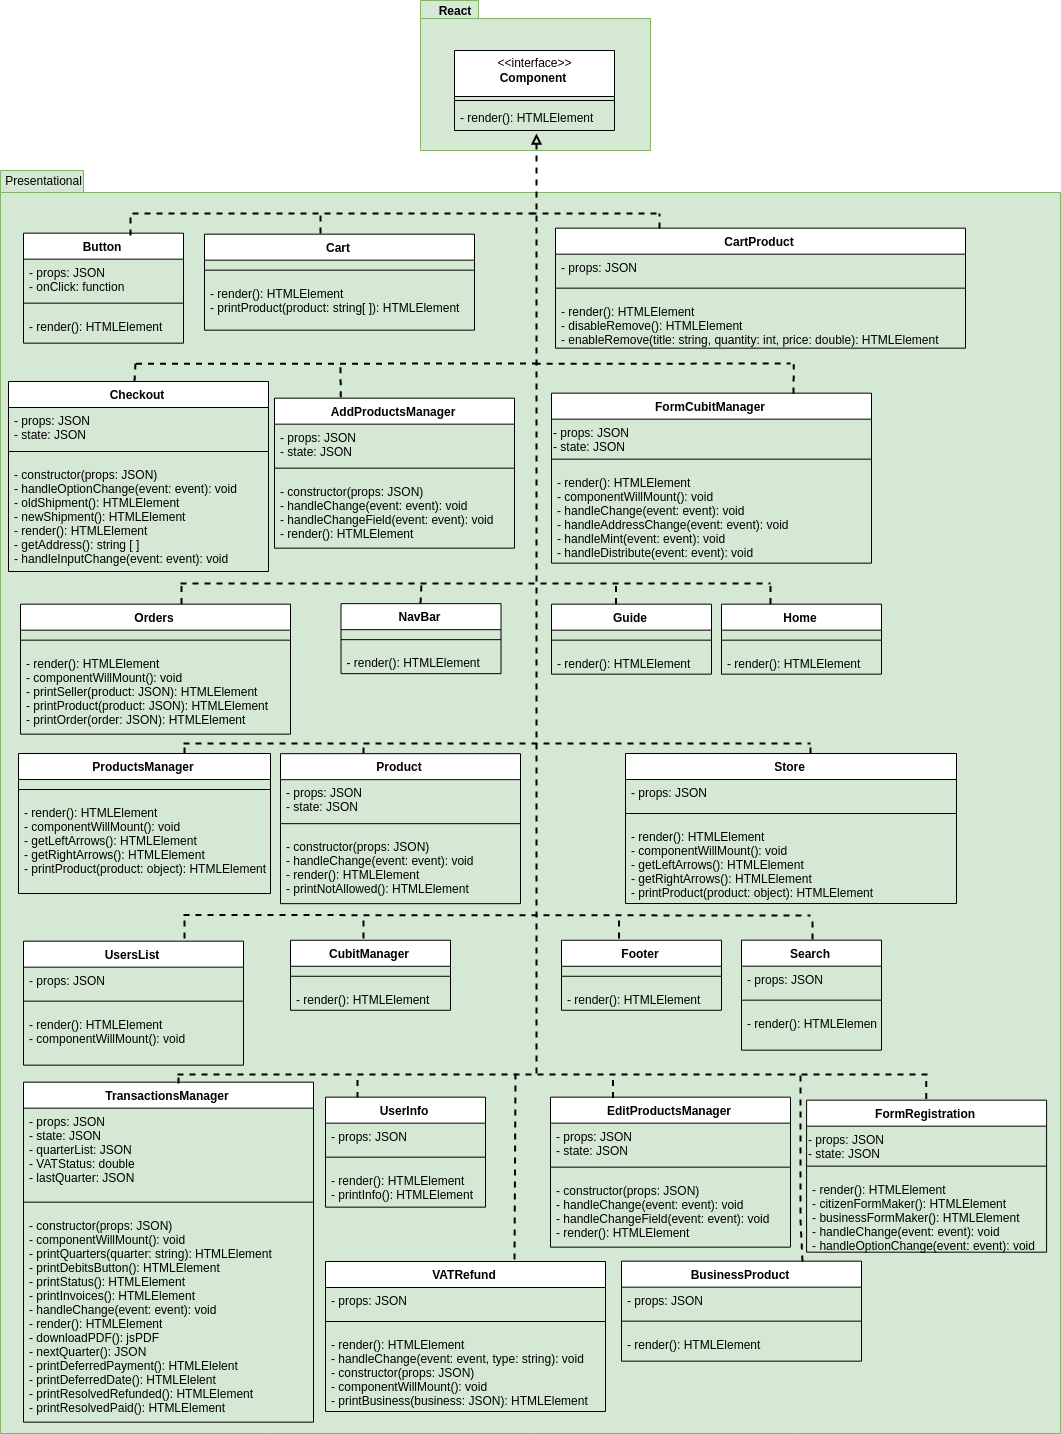
\includegraphics[scale = 0.38]{res/images/Presentational.png}
	\caption{Presentational components}
\end{figure}
\begin{figure}[H]
	\centering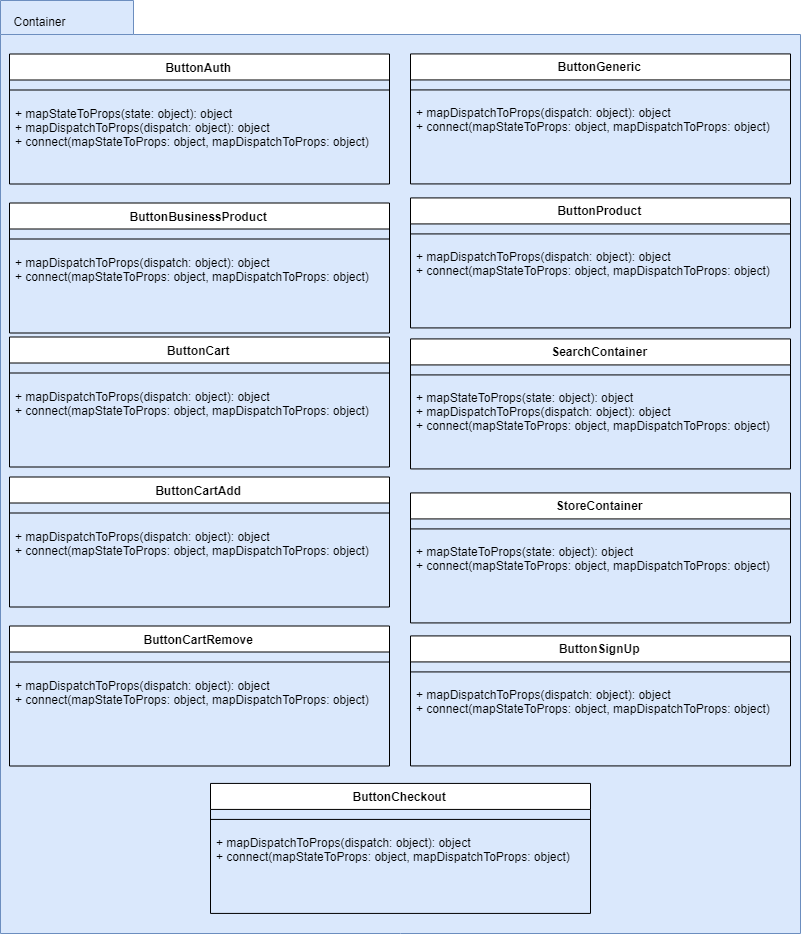
\includegraphics[scale = 0.5]{res/images/Container.png}
	\caption{Container components}
\end{figure}
% \subsection{Collaborations % } if there is one, sequence diag
% \subsection{How to extend} Super optional


\pagebreak
\section{Redux} 
\subsection{Overview}
Redux\glosp is a \texttt{npm} module which manage the entire state of the website from client-side. It consists of:
\begin{itemize}
	\item Actions;
	\item Actions Creators;
	\item Reducers;
	\item Store.
\end{itemize}
When the website is built, a default state for the store is set (it is defined into the reducer JavaScript file).
\subsection{Unidirectional pattern} 
Basically some actions are mapped by \texttt{container components} into specific \texttt{presentational components} through them props with \texttt{Connect(arg1, arg2)} method. When a presentational component request a \texttt{dispatch()} of a specific action, a reducer will complete the request by changing the store and returning a new instance of the application state. Each time the store is changed, the \texttt{Render()} method of displayed components is called.
\texttt{Redux} is the name of the pattern implemented by React and Redux, it is an evolution of \texttt{Flux} pattern, the difference is that Flux uses more than one store.\\
\begin{figure}[H]
	\centering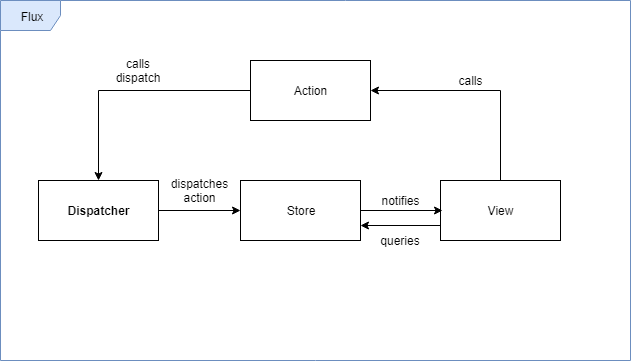
\includegraphics[scale = 0.6]{res/images/Flux.png}
	\caption{Flux pattern}
\end{figure}

\subsection{Actions}
There are twelve different actions inside the \texttt{src/actions/} folder. Each action is called by the \texttt{action creator} when a container component request it's dispatch. Here there is the list of actions and what them do when they are invoked.
\begin{itemize}
	\item \textbf{ACLogin}: it changes the \texttt{logged} state value;
	\item \textbf{ACIncreaseQuantity}: it increases the quantity of a product that is inside the cart, by changing the \texttt{quantity} value of a specified product inside \texttt{cart} state value;
	\item \textbf{ACCartToOrders}: it copies all the content of \texttt{cart} state value to \texttt{ordersList} state value, finally it resets the \texttt{cart} state value;
	\item \textbf{ACSignUp}: it provides to save into the store all of the user informations after they are successfully saved into IPFS\glo;
	\item \textbf{ACAddToCart}: it puts the selected product with selected quantity into \texttt{cart} state value;
	\item \textbf{ACSearch}: it changes \texttt{searchProduct} state value for making a dynamic search inside store page;
	\item \textbf{ACLogout}: it changes the \texttt{logged} state value;
	\item \textbf{ACAddToSelling}: it puts the product into \texttt{selling} state value after it is successfully saved into IPFS;
	\item \textbf{ACReset}: it resets the entire state of application, even if \texttt{redux-persist} is present;
	\item \textbf{ACRemoveFromCart}: it removes the selected product from \texttt{cart} state value;
	\item \textbf{ACDecreaseQuantity}: it decreases the quantity of a product that is inside the cart, by changing the \texttt{quantity} value of a specified product inside \texttt{cart} state value;
	\item \textbf{ACDisableAccount}: it sets a value different from 0 to \texttt{error} state value if something goes wrong, otherwise it sets 0 into \texttt{error} state value.
\end{itemize}
\subsection{Actions Creators}
There are three different type of Actions Creator:
\begin{itemize}
	\item \textbf{Business actions creator}: contains the following functions: 
	\begin{itemize}
		\item getStoreProducts(): generates a list of products on sale and returns it as param by returning a redux action;
		\item getMyProducts(): generates a list of products on sale that were added to sell by current logged business and returns it as param by returning a redux action;
		\item addProduct(): add a product to the store;
		\item modifyProduct(): modify a product to the store;
		\item deleteProduct(): remove a product from the store;
		\item getTotalStoreProduct(): get the number of total products into the store;
		\item getTotalMyProduct(): get the number of total products into the store that were added to sell by current logged business;
		\item getInvoices(): get all the invoices in a quarter;
		\item getBusinessPeriod(): get all the invoices in a quarter related to the current logged business;
		\item payVATPeriod(): execute the instant payment for a quarter to the government;
		\item putOnHoldVATPeriod(): defer the debt of a quarter to the next quarter.
	\end{itemize}
	\item \textbf{User actions creator};
	\item \textbf{Government actions creator}.
\end{itemize}
Each of them interacts with Facade (cf. §9) and returns to the related contanier a specific action otherwise rejects an error.
\subsection{Reducers}
\begin{itemize}
	\item \textbf{ReducerAuth}: it makes the dispatch of the actions inside:
	\begin{itemize}
		\item ACLogin;
		\item ACLogout;
		\item ACSignUp;
		\item ACReset.
	\end{itemize}
	\item \textbf{ReducerSearch}: it makes the dispatch of search action;
	\item \textbf{ReducerCart}: it makes the dispatch of the actions inside:
	\begin{itemize}
		\item ACIncreaseQuantity;
		\item ACDecreaseQuantity;
		\item ACCartToOrders;
		\item ACAddToCart;
		\item ACAddToSelling;
		\item ACRemoveFromCart.
	\end{itemize}
	\item \textbf{ReducerGovernment}: it makes the dispatch of disableAccount action.
\end{itemize}
\subsection{Store}
It's configuration resides into root reducer file, the initial configuration is:
\begin{itemize}
	\item logged: false;
	\item user: null;
	\item searchProduct: "";
	\item cart: [ ];
	\item pending: [ ];
	\item ordersList: [ ];
	\item error: 0.
\end{itemize}
Each time the \texttt{reset} action is dispatched from it's reducer, the initial configuration of the store is set.

\subsection{Redux-Persist}
It is a \texttt{npm} module used for maintaining the current store even if the user leaves the website. It is browser-locally saved, so if a user will enter into the website from another device or from another browser, the store will be set with default values. It has a blacklist for bypassing some values, in this way reloading the website, these values will not be saved (the blacklist is defined into reducer JavaScript file).

\begin{landscape}
	\subsection{UML} 
	
	\begin{figure}[H]
		\centering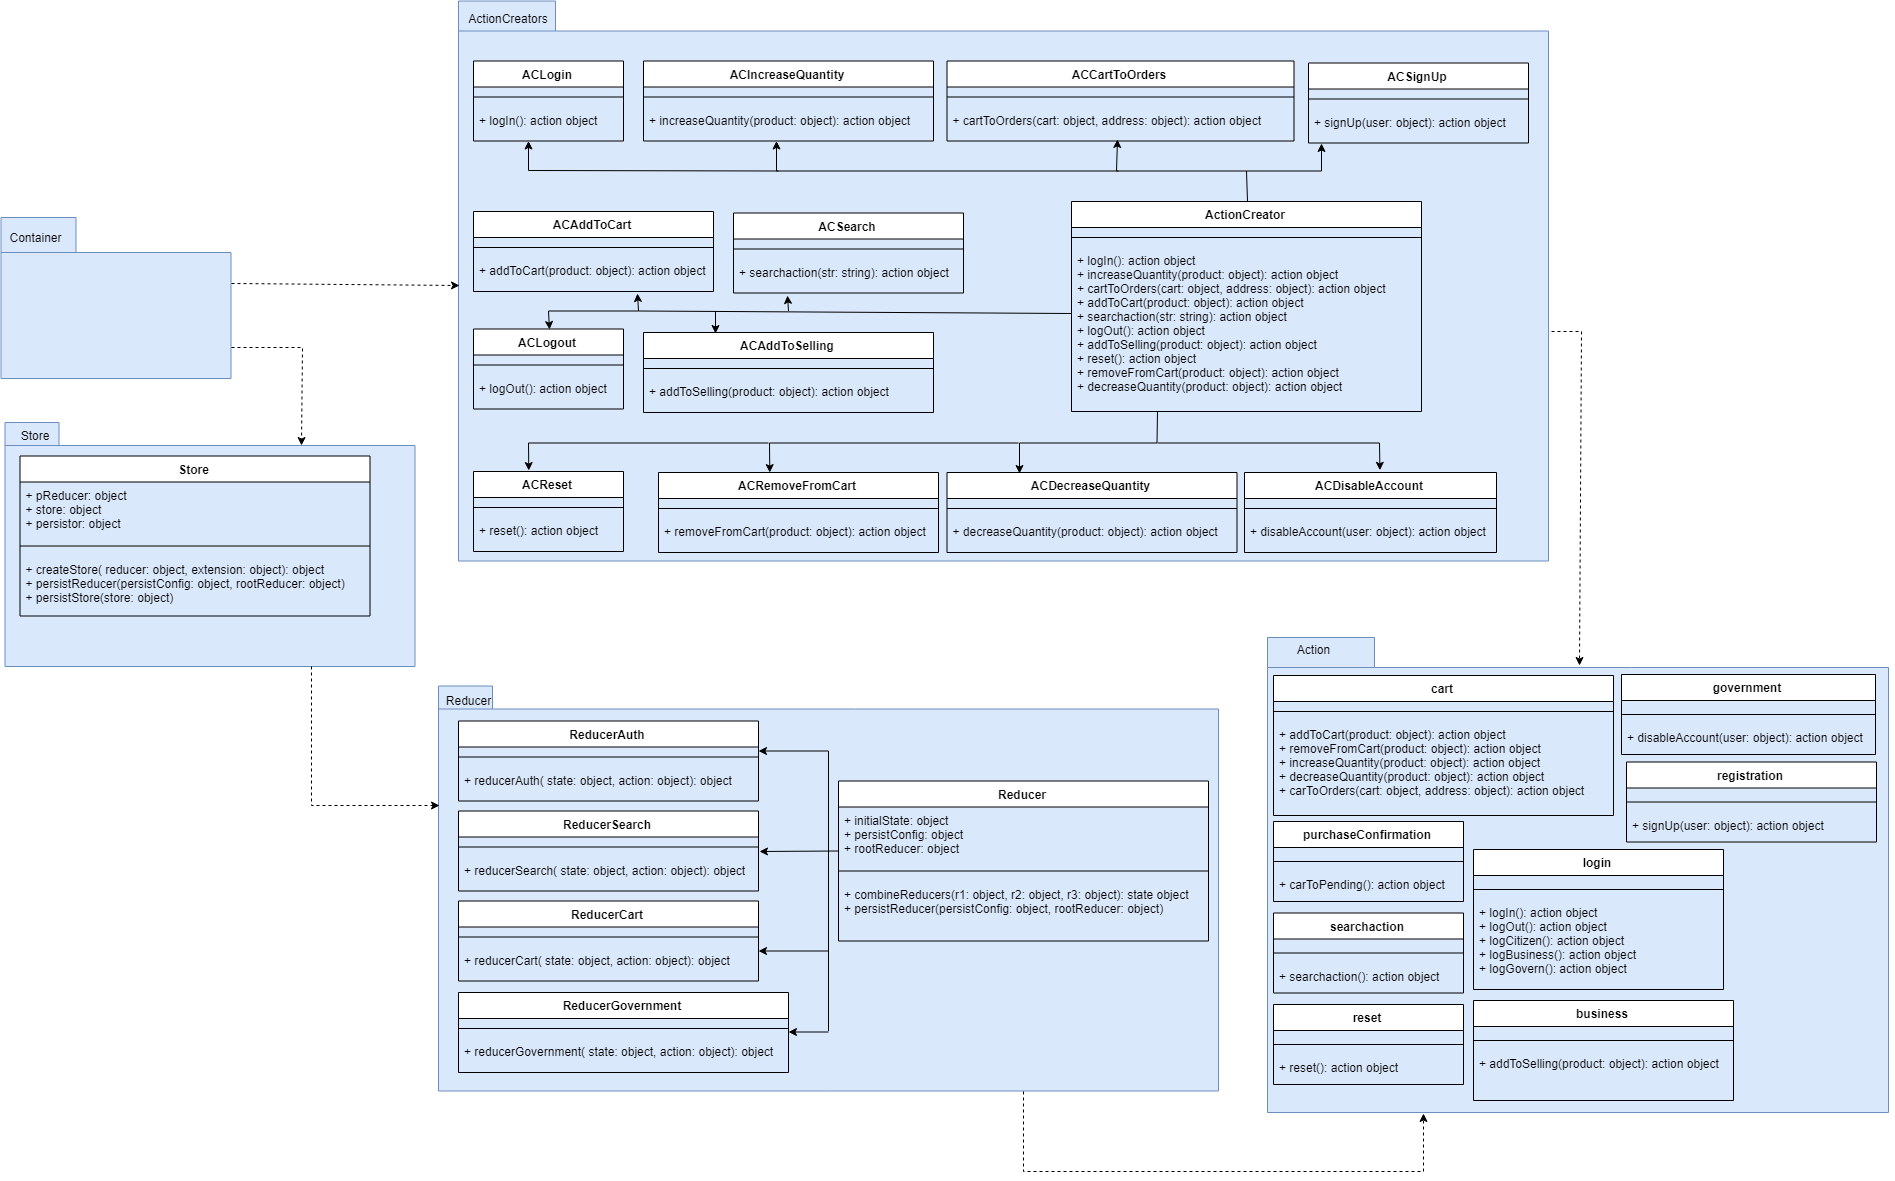
\includegraphics[scale = 0.3]{res/images/ReduxDiagram.png}
		\caption{Redux architecture}
	\end{figure}
\end{landscape}

\pagebreak
\section{Web3} 
web3.js is a collection of libraries that allows you to interact with a local or remote Ethereum node. Moreover, it is able to communicate with MetaMask, which is the add-on for Chrome and Mozilla Firefox that lets the user manage his Ethereum wallet and confirm transactions in an intuitive and secure way. Using MetaMask we offer secure payments and automatic login to \textit{Soldino}.
\subsection{Architecture overview}
To interact with web3 library calls we organized the \texttt{web3functions} package into five different modules:
\begin{figure}[h]
	\centering
	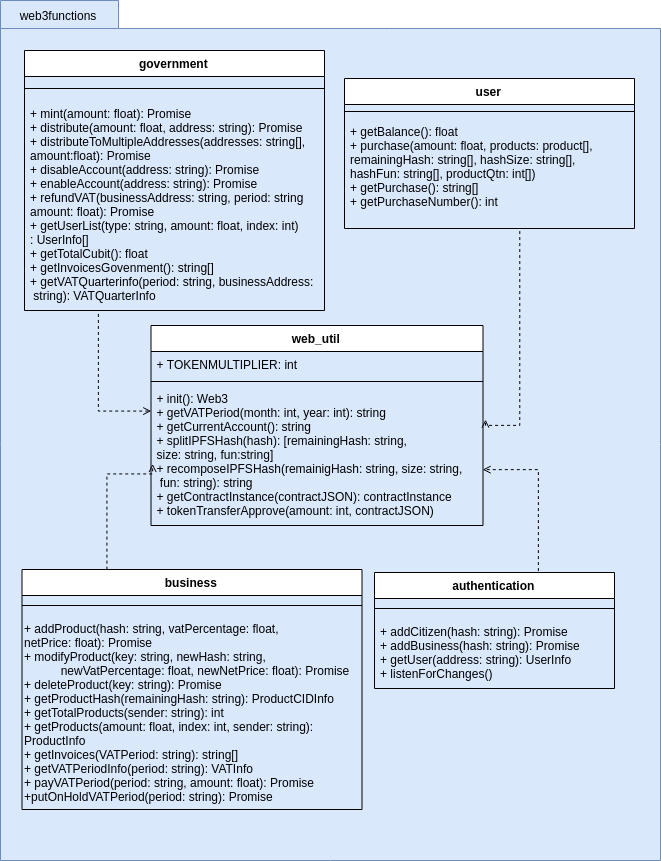
\includegraphics[scale=0.65]{res/images/web3.png}
	\caption{Class diagram of the \texttt{web3functions} package}
\end{figure}
\subsection{Methods}

The five modules groups some methods that are responsible for setting data to Ethereum or retrieving them from the blockchain.

\subsubsection{web\_utils}
This module groups some utility functions that are used by the other modules to make the web3 call easier:
\begin{itemize}
	\item \textbf{getWeb3}: tries to get an instance of a web3 object, which will be used to make all the web3 calls. Specifically, it tries to get the web3 object instance injected by MetaMask, if this is possible, otherwise it returns an error;
	\item \textbf{splitIPFSHash}: a function that converts the base58 string representing the IPFS CID into three variables, since this information is saved in this way in the blockchain for cost and scalability reasons;
	\item \textbf{recomposeIPFSHash}: it's the the inverse of the function descripted above, it recomposes the IPFS CID.
\end{itemize} 

\subsubsection{authentication}
This module manages the registration and login of all the types of users:
\begin{itemize}
	\item \textbf{addCitizen}: registers a new citizen using the Ethereum address provided by MetaMask, and saves the IPFS CID, that represents the related information saved in the peer-to-peer network;
	\item \textbf{addBusiness}: registers a new business using the Ethereum address provided by MetaMask, and saves the IPFS CID, that represents the related information saved in the peer-to-peer network;
	\item \textbf{getUser}: returns the IPFS CID corresponding to the current Ethereum address of the user provided by MetaMask.
\end{itemize}
\subsubsection{user}
This module manages the common functionality offered to citizen and business:
\begin{itemize}
	\item \textbf{buy}: manage a new order making the user transfer the due amount of \textit{Cubit} to the target companies;
	\item \textbf{getSalesOrders}: gets the IPFS CID related to an order. With the IPFS CID all the order's information can be retreived.
\end{itemize}
\subsubsection{business}
This module manages the functionality offered to business:
\begin{itemize}
	\item \textbf{getSalesInvoices}: returns an array containing all the IPFS CID related to the sales invoices;
	\item \textbf{getPurchaseInvoices}: returns an array containing all the IPFS CID related to the purchases invoices;
	
	\item \textbf{insertProduct}: inserts the product passed as JSON in the Ethereum blockchain; 
	\item \textbf{insertOrder}: creates a new order made of the product passed to the function;
	\item \textbf{insertVAT}: inserts the VAT information related to the order passed to the function;
	\item \textbf{payVAT}: allows a business to pay the VAT owed by the government related to a particular VAT quarter;
	\item \textbf{postponeVATPayment}: allows a business to postpone the VAT payment to the government related to a particular VAT quarter;
	\item \textbf{modifyProduct}: allows a business to modify one of its product that was previously been added;
	\item \textbf{deleteProduct}: allows a business to delete one of its products that were previously been added. The product will not be shown in the store anymore.
\end{itemize}
\subsubsection{government}
Module to manage the common functionality offered to the government:
\begin{itemize}
	\item \textbf{mint}: lets the government mint a specific amount of \textit{Cubit}. This amount is deposited in the government account;
	\item \textbf{distribute}: lets the government transfer a specific amount of \textit{Cubit} from his own account to a target account;
	\item \textbf{disableAccount}: lets the government set the state of the target account to "disabled". The target account will not be able to use the platform until it has been restored;
	\item \textbf{modifyProduct}: lets the government set the state of the target account to "enabled". The target account will be able to use the platform;
	\item \textbf{refundVAT}: lets the government refund a business. The owed amount of \textit{Cubit}, related to a specific VAT quarter, will be transferred to the target business.
\end{itemize}


\pagebreak
\section{IPFS} 

It is well known that the Ethereum blockchain is not suited for saving data. You just need to know that for hypothetically uploading a file on Ethereum, you would have to pay about 2\$ per kilobyte. 
\\
For these reasons, we adopted the InterPlanetary File System (IPFS) protocol, to store all the information that is not involved in VAT management, in the homonymous peer-to-peer network. Specifically, for security purposes, all the data used to make payments between the clients are exclusively stored in the Ethereum blockchain. All the remaining data, such as not sensitive clients' data, products' data, orders' data, are stored into IPFS since it is a free and distributed technology born with the aim of sharing every kind of content.


\subsection{Architecture overview}

To establish a connection to the IPFS network, we developed a small package, that is responsible for hiding the IPFS connection implementation (\texttt{ipfs-mini} API). The available interface contains two methods: one for adding new data into the blockchain, and the other one for retrieving them starting from the IPFS content identifier (CID).
\begin{figure}[h]
	\centering
	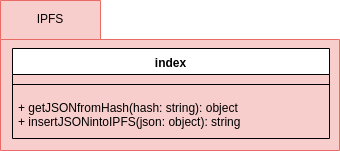
\includegraphics[scale=0.6]{res/images/IPFS.png}
	\caption{Class diagram of the IPFS package}
\end{figure}
\subsection{Methods}
The package provides the following methods:
\begin{itemize}
	\item \textbf{getJSONfromHash}: it uses the \texttt{ipfs-mini} API to retreive the JSON object corresponding to the passed IPFS CID;
	\item \textbf{insertJSONintoIPFS}: it uses the \texttt{ipfs-mini} API to upload the JSON passed to the function, then returns the IPFS CID.
\end{itemize}



\pagebreak
\section{Facade} 

\subsection{Architecture overview}

Since most of the operations include the interaction with both web3funcions and IPFS packages, we provide a third package, facade, with the aim of hiding the web3 and IPFS layers. This package executes function calls, in the suitable order, to the other two packages, saving and retrieving data from both IPFS and Ethereum.

\begin{figure}[h]
	\centering
	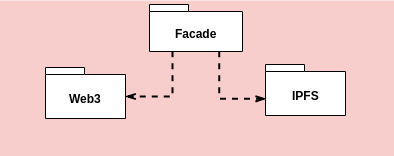
\includegraphics[scale=0.6]{res/images/facade.png}
	\caption{Package diagram with the interaction between facade-web3-IPFS}
\end{figure}

\subsection{Methods}

All the methods describe in the picture below consists of two different steps:
\begin{itemize}
	\item \textbf{setter}: firstly the data is stored to IPFS, then it is stored to Ethereum with related IPFS CID;
	\item \textbf{getter}: firstly the IPFS CID is retrived from web3. The CID is then used to get the 
\end{itemize}
\begin{figure}[H]
	\centering
	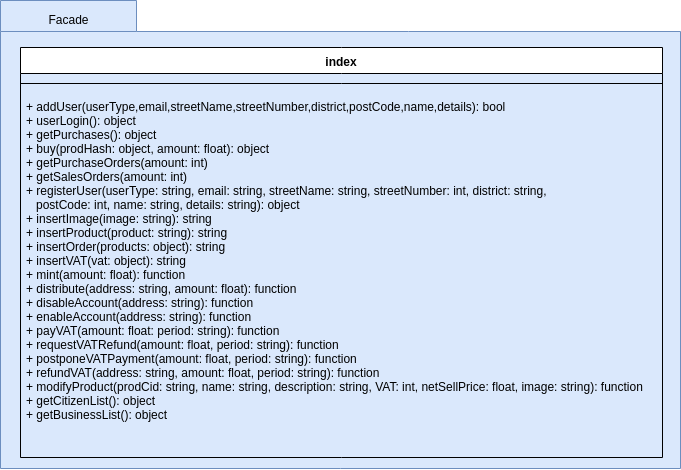
\includegraphics[scale=0.55]{res/images/facade-package.png}
	\caption{Class diagram of the facade package}
\end{figure}

\noindent Since the methods are just a combination of the already described methods of the web3 and IPFS packages, we omit their description.



\pagebreak
\section{Solidity}
% i nomi delle sezioni sono indicativi, non tassativi

\subsection{Overview}
\subsection{Contracts} % described with class diagrams
\subsection{Collaborations} % significative interactions described through sequence diagrams
\subsection{How to extend} % upgradability; manager attachs and detachs contracts



%\pagebreak
%\section{Testing}
% questo cap effettivamente ha questo scopo nei 353 (2 pagine). In sostanza parla piu` di metriche che di test
This chapter shows how to
\begin{itemize}
	\item test the javascript and solidity code automatically;
	\item check if the code syntax is complied to the rules given.
\end{itemize}
\subsection{Test in Javascript Code}
%PLACEHOLDER
\subsection{Test Solidity Code}
\subsection{Code Coverage}
\textbf{Note}: Not available for Windows. \\
To run test coverage open new shell into the \textit{Soldino} project directory and run: \\ \\ \texttt{npm run coverage}. \\ \\ After a while it will show you every successfully tests and costs of transactions. The port that is used for test newtork is 8545.

\pagebreak
\appendix
\section{Glossary}
	\subsection*{C}
	\addcontentsline{toc}{subsection}{C}
		\subsubsection*{Cubit}
		Cubit is the custom Ethereum currency of \textit{Soldino}, it has the value 
		of 1\euro. All prices shown are in Cubits. The Government can mint 
		and distribute Cubits to the platform's users.
		\subsubsection*{CC}
		Short version of Cubit, see Cubit above.
	
	\subsection*{D}
	\addcontentsline{toc}{subsection}{D}
		\subsubsection*{Deferred payment}
		Businesses can choose to not pay their due taxes immediately and pay it 
		later.
		\subsubsection*{Digital wallet}
		Digital wallets are where virtual currency is stored.
	
	\subsection*{E}
	\addcontentsline{toc}{subsection}{E}
		\subsubsection*{Ether}
		Ether is the currency of Ethereum.
		\subsubsection*{Ethereum}
		Ethereum is an open software platform based on blockchain technology 
		that enables developers to build and deploy decentralized applications.
		
	\subsection*{G}
	\addcontentsline{toc}{subsection}{G}
		\subsubsection*{Gas}
		Gas is the cost of transactions made on the Etehreum network. It is 
		measured in GWEI which is a billionth of an Ether.
		
	\subsection*{M}
	\addcontentsline{toc}{subsection}{M}
		\subsubsection*{MetaMask}
		MetaMask is a Plug-in available for Chrome, Firefix, Opera and Brave that 
		allows you to interact with the Ethereum network without hosting a node 
		and create multiple digital wallets\glo.
		\\It is required to use in \textit{Soldino}.
		
	\subsection*{P}
		\addcontentsline{toc}{subsection}{E}
		\subsubsection*{Product}
		Products include both goods and services.
		
	\subsection*{V}
	\addcontentsline{toc}{subsection}{V}
		\subsubsection*{VAT}
		VAT or value-added tax is a type of tax that is assessed incrementally, 
		based on the increase in value of a product or service. The VAT 
		percentage is chosen by the product's seller.


\end{document}
